\documentclass{gadsescript}

\settitle{Encoding II, Algorithms and Data Structures}
\setsubtitle{Elias Gestrich}

\begin{document}
\maketitle
\section*{\textbf{Exercise 1:} IEE 754 Number format}
\begin{enumerate}[label=\alph*)]
	\item first bit: $ 1 $ $ \rightarrow $ negative\\
		following $ 8 $ bits: $ 10000001 = \binnum[8]{0111 1111} + \binnum{10} $ $ \rightarrow $ Exponent is $ \binnum{10} $\\
		other bits: $ {101 0000 0000 0000 0000 0000} \rightarrow $ Mantissa is $ \binnum{1.101} $\\
		$\implies$ $1 1000 0001 10100000000000000000000 = - \binnum{1.101} \times \binnum{10}^{\binnum{10}} = -\binnum{1101.1} = -\decnum{13.5} $
	\item positive: first bit = 0\\
		$\decnum{20.5} =  \binnum{10100.1} \rightarrow $ mantissa: $ 01001000000000000000000 $, exponent: $\binnum[8]{111 1111} + \binnum{100} = \binnum[8]{1000 0011} $\\
		$\implies 0 1000 0011 010 0100 0000 0000 0000 0000$
\end{enumerate}

\section*{Exercise 2: ASCII}
\begin{enumerate}[label=\alph*)]
	\item S = $ \hexnum{53} $, k = $ \hexnum{6B} $, I = $ \hexnum{49} $: ``SkI'' = $ \hexnum{536B49} = \binnum{0101 0011 0110 1011 0100 1001} $
\end{enumerate}

\section*{Exercise 3: Binary Search Trees}
\begin{enumerate}[label=\alph*)]
	\item insert(11)\\
		empty tree: 11 becomes root\\
		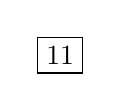
\begin{tikzpicture}
			\node{\fbox{11}};
		\end{tikzpicture}\\[4pt]
		insert(10)\\
		$ 10 < 11 $\\
		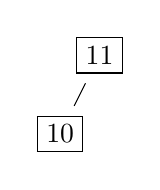
\begin{tikzpicture}
			\node{\fbox{11}} [level distance = 1cm]
			child {node [xshift = -0.5cm] {\fbox{10}}};
		\end{tikzpicture}\\[4pt]
		insert(9)\\
		$ 9 < 11 \rightarrow 9 < 10 $\\
		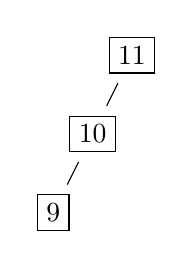
\begin{tikzpicture}
			\node{\fbox{11}} [level distance = 1cm]
				child {node [xshift = -0.5cm] {\fbox{10}}
					child {node [xshift = -0.5cm] {\fbox{9}} }
				}
			;
		\end{tikzpicture}\\[4pt]
		insert(6)\\
		$ 6 < 11 \rightarrow 6 < 10 \rightarrow 6 < 9 $\\
		\begin{tikzpicture}
			\node{\fbox{11}} [level distance = 1cm]
				child {node [xshift = -0.5cm] {\fbox{10}}
					child {node [xshift = -0.5cm] {\fbox{9}}
						child {node[xshift = -0.5cm] {\fbox{6}} }
					}
				}
			;
		\end{tikzpicture}\\[4pt]
		insert(14)\\
		$ 14 > 11 $\\
		\begin{tikzpicture}
			\node{\fbox{11}} [level distance = 1cm]
				child {node {\fbox{10}}
					child {node [xshift = -0.5cm] {\fbox{9}}
						child {node[xshift = -0.5cm] {\fbox{6}} }
					}
				}
				child {node {\fbox{14}} }
			;
		\end{tikzpicture}\\[4pt]
		insert(12)\\
		$ 12 > 11 \rightarrow 12 < 14$\\
		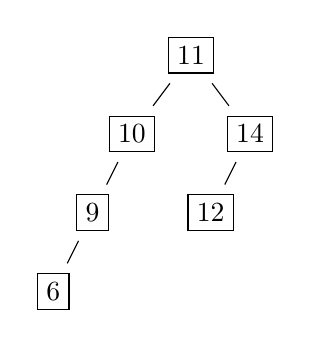
\begin{tikzpicture}
			\node{\fbox{11}} [level distance = 1cm]
				child {node {\fbox{10}}
					child {node [xshift = -0.5cm] {\fbox{9}}
						child {node[xshift = -0.5cm] {\fbox{6}} }
					}
				}
				child {node {\fbox{14}}
					child {node [xshift = -0.5cm] {\fbox{12}} }
				}
			;
		\end{tikzpicture}\\[4pt]
		insert(15)\\
		$ 15 > 11 \rightarrow 15 > 14$\\
		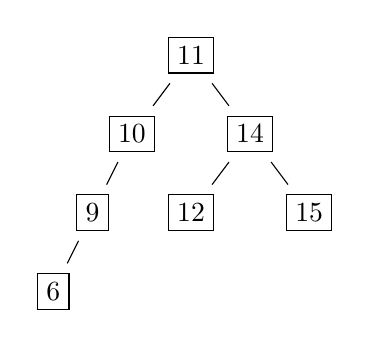
\begin{tikzpicture}
			\node{\fbox{11}} [level distance = 1cm]
				child {node {\fbox{10}}
					child {node [xshift = -0.5cm] {\fbox{9}}
						child {node[xshift = -0.5cm] {\fbox{6}} }
					}
				}
				child {node {\fbox{14}}
					child {node {\fbox{12}} }
					child {node {\fbox{15}} }
				}
			;
		\end{tikzpicture}\\[4pt]
		remove(12) $ \rightarrow $ 12 has no child:
		\begin{tikzpicture}
			\node{\fbox{11}} [level distance = 1cm]
				child {node {\fbox{10}}
					child {node [xshift = -0.5cm] {\fbox{9}}
						child {node[xshift = -0.5cm] {\fbox{6}} }
					}
				}
				child {node {\fbox{14}}
					child {node [xshift = 0.5cm]{\fbox{15}} }
				}
			;
		\end{tikzpicture}\\[4pt]
		remove(11) $ \rightarrow $ 11 has two childs: replace 11 with the most right element of the left child (the 10) and remove the child, because 10 has one child on the left side move this child to the left side of the root:\\
		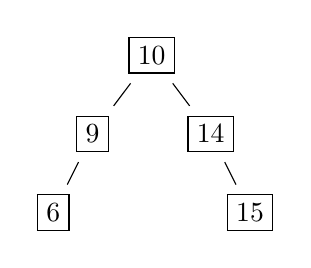
\begin{tikzpicture}
			\node{\fbox{10}} [level distance = 1cm]
				child {node {\fbox{9}}
					child {node[xshift = -0.5cm] {\fbox{6}} }
				}
				child {node {\fbox{14}}
					child {node [xshift = 0.5cm]{\fbox{15}} }
				}
			;
		\end{tikzpicture}\\[4pt]
\end{enumerate}

\section*{Exercise 4: Hashing}
\begin{enumerate}[label=\alph*)]
	\item 13???
	\item~\\
		\begin{tabular}{c|l}
			0 & $\rightarrow$ 7\\\hline
			1 & $\rightarrow$ 6\\\hline
			2 & $\rightarrow$ 5\\\hline
			3 & $\rightarrow$ 8\\\hline
			4 & $\rightarrow$ (7 collision $\rightarrow$ +7) 14\\\hline
			5 & $\rightarrow$ 1\\\hline
			6 & $\rightarrow$ 10\\\hline
			7 & $\rightarrow$ (5 collision $\rightarrow$ + 31) 36\\\hline
			8 & $\rightarrow$ 12\\\hline
			9 & $\rightarrow$ 3\\\hline
			10 & $\rightarrow$ (1 collision $\rightarrow$ + 27) 28\\\hline
			11 & $\rightarrow$ (8 collision $\rightarrow$ + 34) 42\\
		\end{tabular}
\end{enumerate}

\end{document}
